\documentclass[t,compress,11pt,xcolor=dvipsnames]{beamer}
\usefonttheme[onlymath]{serif}
\usetheme{Ilmenau}
\definecolor{LHCblue}{RGB}{4, 114, 255}
\usecolortheme[named=LHCblue]{structure}
\usepackage[bars]{beamerthemetree} % Beamer theme v 2.2
\usepackage{multicol}
\usepackage{lmodern}
\usepackage{lipsum}
\usepackage{marvosym}
\title{ CS251 Project Report by Group 12.}
\author[Pramod  \&  Basith \& Nikhileswar  ]
{
   \texorpdfstring{
        \begin{columns}
            \column{.30\linewidth}
            \centering
            Pramod \\
            140050076 \\
            {140050076@itb.ac.in}
            \column{.30\linewidth}
            \centering
            Basith \\
             140050070 \\
             {140050070@itb.ac.in}
            \column{.30\linewidth}
            \centering
            Nikhileswar \\
             140050074 \\
            {140050074@itb.ac.in}
        \end{columns}
   }
   {John Doe \& Jane Doe}
   }
\date{\today}

\begin{document}
\section{Aims}
\begin{frame}
\frametitle{Aims}
During the beggining of project our idea was to make this simulation and synchronize it such that both balls from left,right part of system collide. \\~\\
After completion of basic simulation we thought the whole purpose of the simulation was for nothing!!,so we added extra objects like dominos,revolving platforms to make it to do something.\\~\\
Finally the intial balls along with additional objects are  used to make all the 8balls fall into the basket type of system in the middle.\\~\\
The system simulation in left and right parts are in synchroniztion.Both the balls reach ground dominos same time.
\end{frame}
\section{Description}
\begin{frame}
\frametitle{Description}
\begin{columns}[t]
\column{0.3\textwidth}
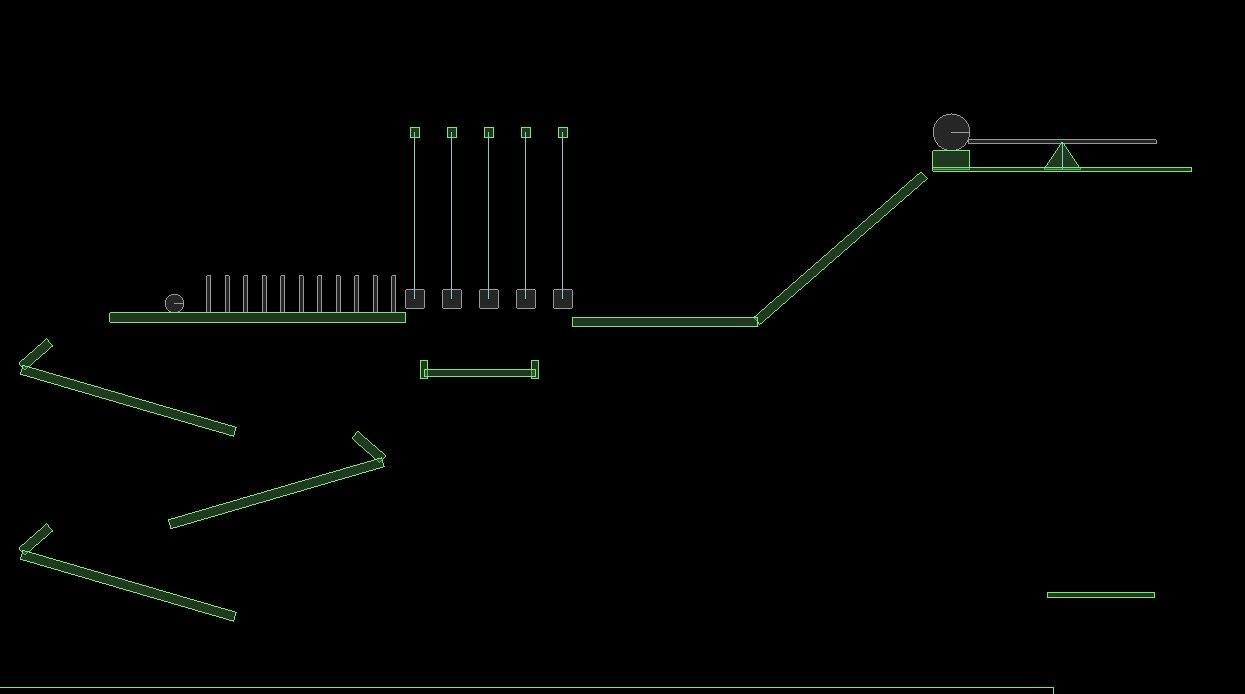
\includegraphics[width=4cm,height=3cm]{left.jpg}
\column{0.3\textwidth}
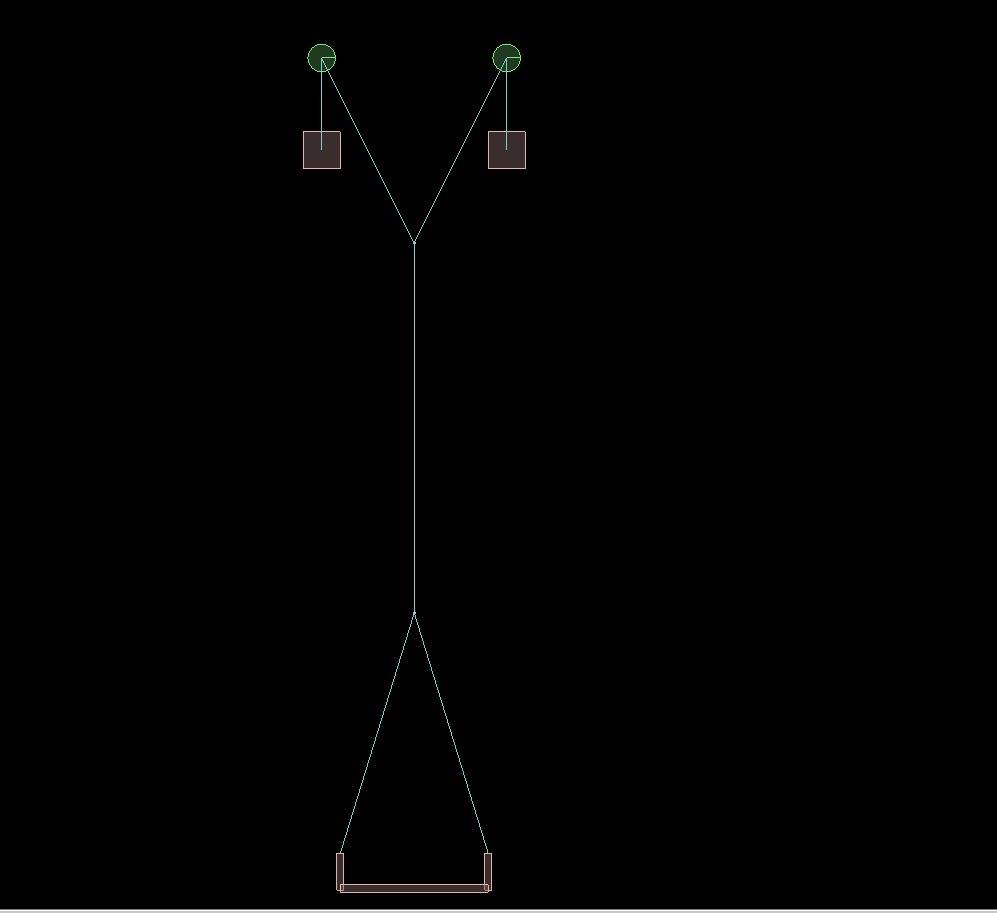
\includegraphics[width=4cm,height=3cm]{middle.jpg}
\column{0.4\textwidth}
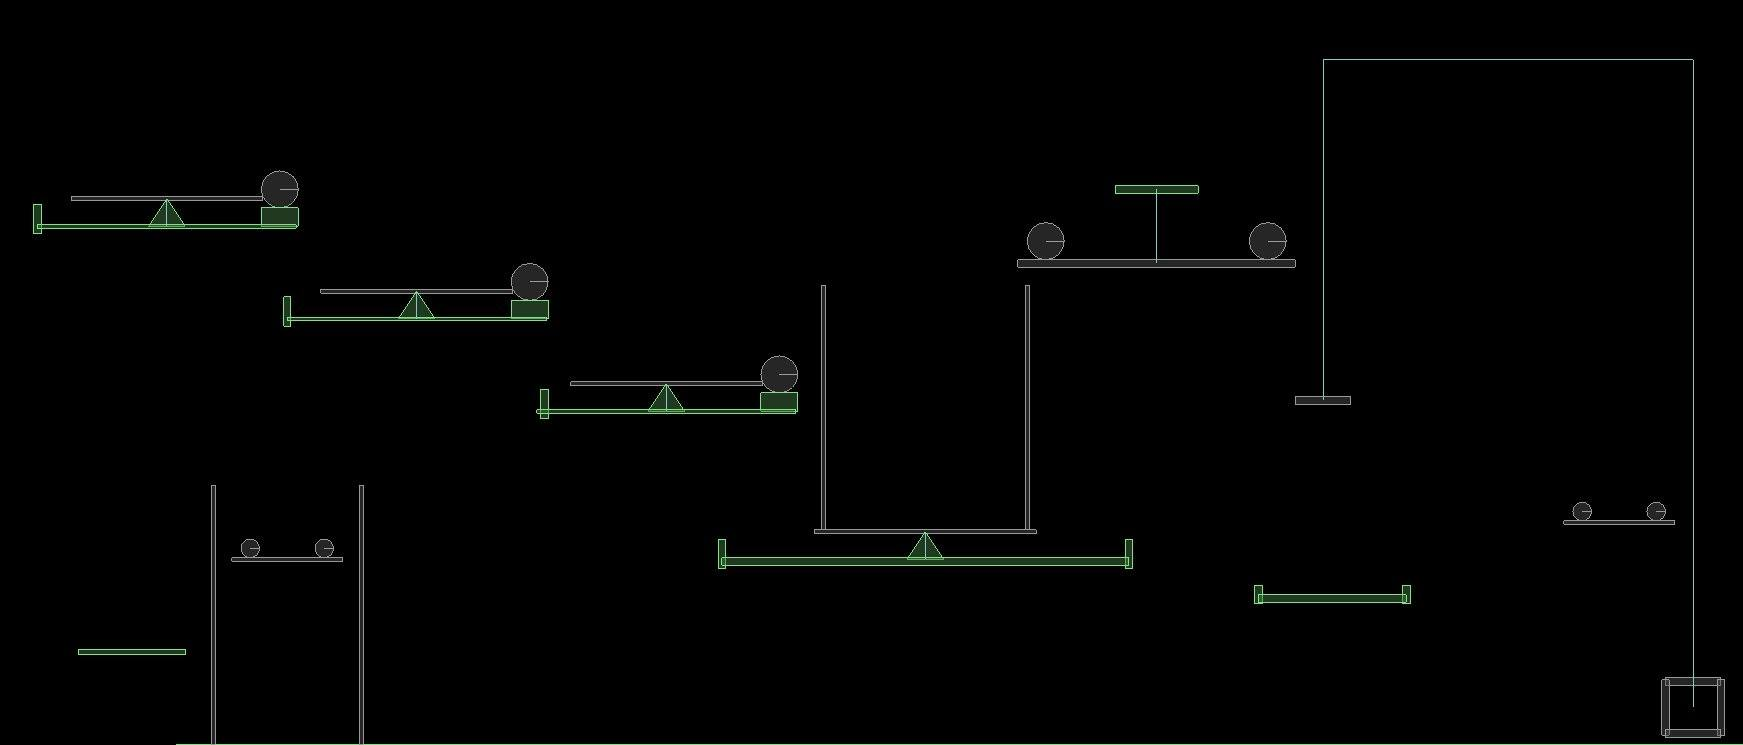
\includegraphics[width=4cm,height=3cm]{right.jpg}
\end{columns}
The only deviation from our original plan was the failure to implement sccisors kind of object into our system.
We tried by using cotactlistener function and then deleting the joints,but we got the basic idea but due to time bound we were unable to complete it.
\end{frame}
\section{left}
\begin{frame}
\frametitle{Left}
\begin{center}
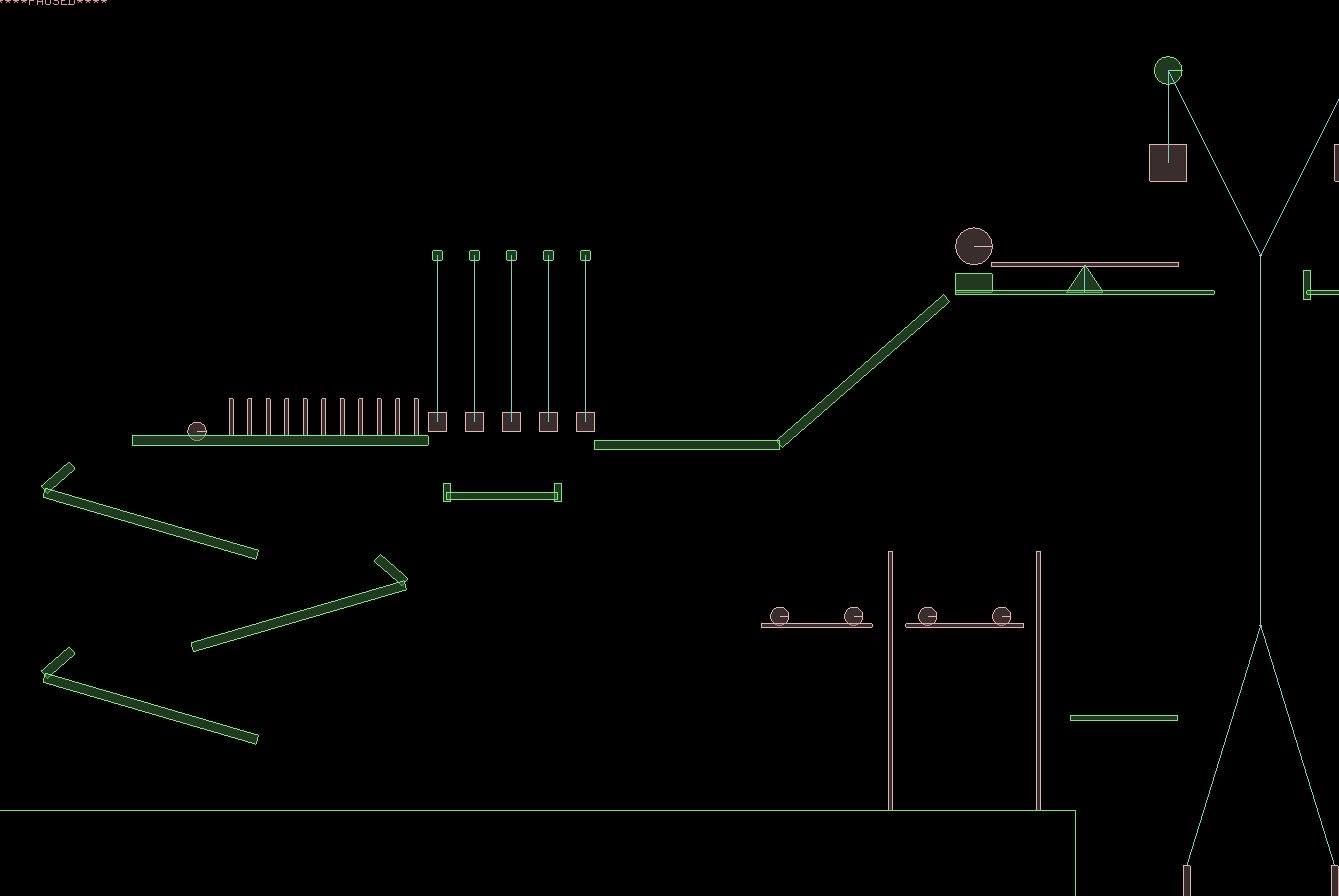
\includegraphics[width=4cm,height=3cm]{left1}
\end{center}
The box hits the plank on the wedge and the ball on the other side of the plank moves down and hits the pendulum.The pendulums disturb the dominoes which in turn disturbs ball on the plane.The ball moves down through the inclined planes and hits the long dominoes which 
disturbs the balls on the revolving plank which go into the basket  \\~\\
\end{frame}
\section{right}
\begin{frame}
\frametitle{Right}
\begin{center}
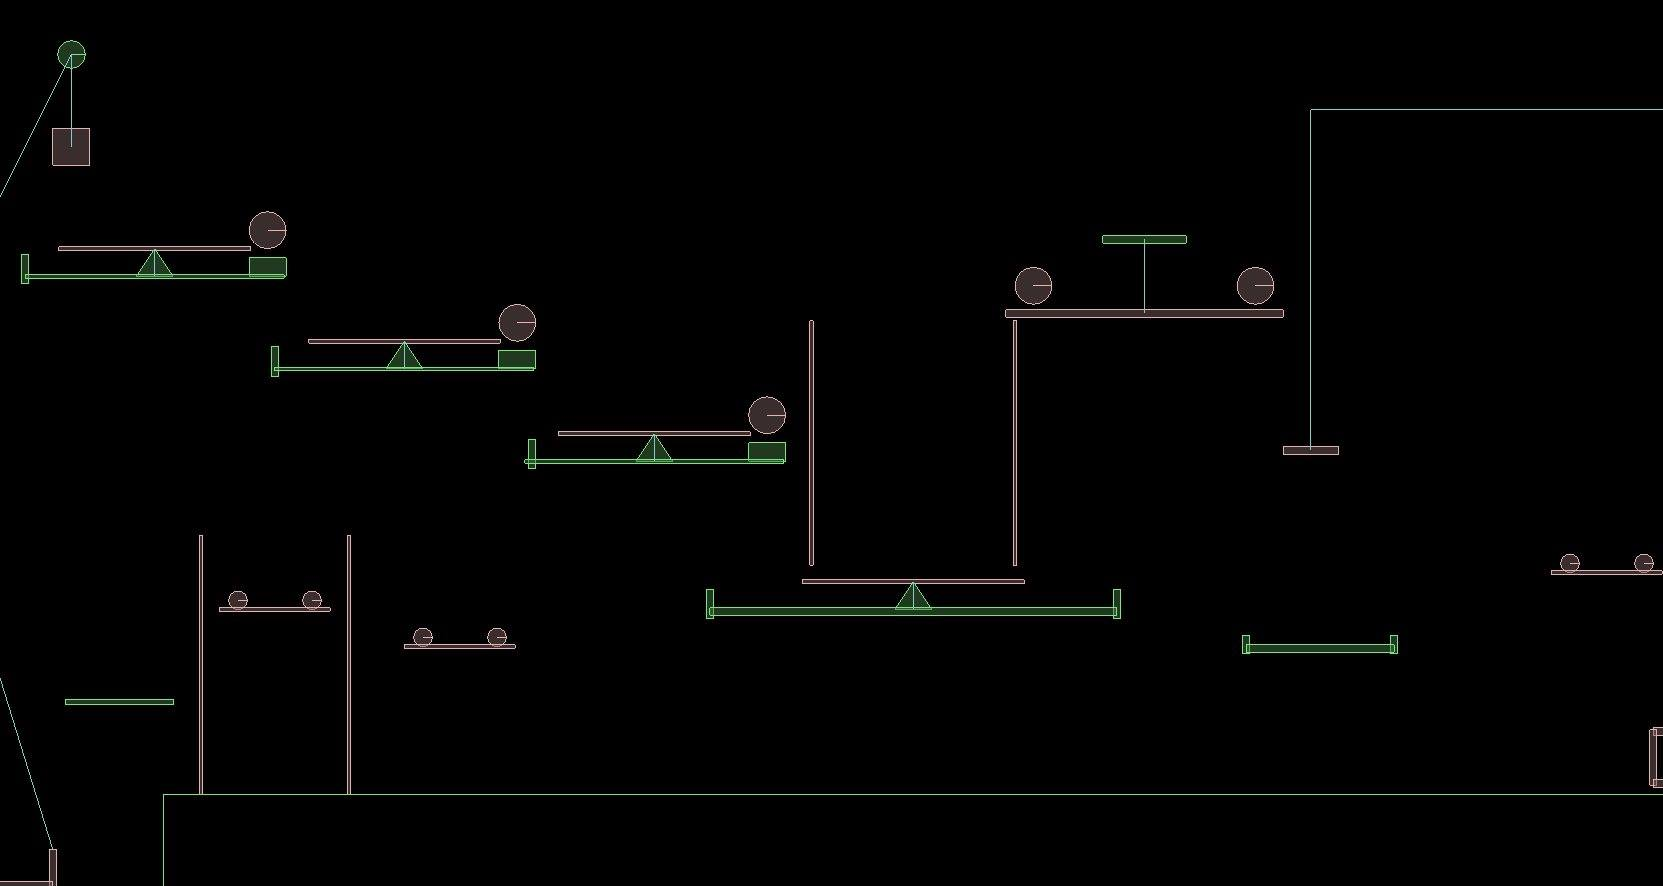
\includegraphics[width=4cm,height=3.0cm]{right1}
\end{center}
The box hits the plank on wedge the balls move down along and they cause disturbance in see-saw with dominoes and the dominoes hit the revolving platform and ball falls on bar of the pulley and the other side of the pulley disturbs the small revolving platform.One of these balls move to left due to collison and it collides with long dominoes,thus making the balls to move into the basket.
\end{frame}
\section{Profiling}
\begin{frame}
\frametitle{About Profiling}
Profing is very useful to write optimised programs.It gives the description of time consumed by different functions in our code so that we can understand which function to be optimised.
The flat profile of analysis.txt shows that all the function calls are taking vary less time.Therefore there is no need to optimise any particular function. However we user -O3 compiling option to optimise. The result of which is shown in analysis updated.txt .There we observe that the percentage of time for some of the function calls have increased which occurs because many of the functions have been optimised which can be known by checking the number of functions listed in the call graphs of both text files so the remaining time is distributed among the functions which results in the increased percentage oftime of those particular functions.
\end{frame}
\end{document}
